\chapter{Conceitos}

% \setlength\epigraphwidth{1\textwidth}
% \setlength\epigraphrule{0pt} % no line between
% \setlength\beforeepigraphskip{1\baselineskip} % space before and after epigraph
% \setlength\afterepigraphskip{2\baselineskip}
% \renewcommand*{\textflush}{flushright}
% \renewcommand*{\epigraphsize}{\normalsize\itshape}
% \epigraph{O que significam as cores da bandeira nacional? \\ O verde é a esperança, né? O amarelo sei lá, desespero. O azul eu não sei. \\ --- \small{Benedita da Conceição, 69, Aposentada}}


\label{cap:conceitos}
Abordamos nesse capítulo as técnicas de síntese desenvolvidas historicamente até o alcance da síntese neural, foco desse trabalho. O intuito de discutir a evolução de técnicas históricas é observar o desenvolvimento de possíveis estratégias que possam ser permutáveis entre técnicas e quais preocupações buscavam resolver. Como comentado anteriormente, na discussão de outras técnicas acabamos permeando outras áreas de pesquisa com intercessões nos assuntos que nos interessam mas que permeiam outros objetivos em suas respectivas áreas. Esses tópicos, em particular, são abordados de maneira superficial já que existem motivos próprios para decisões dentro de cada atividade e, ciente dessas possibilidades, podemos alinhar respectivamente os modelos para interação ótima. Trazemos os modelos mais recentes de síntese de fala neural e discutimos as diferenças entre a \textbf{adaptação de falante} e o \textbf{aprendizado de parâmetros para cada falante}, que são as estratégias mais populares. Trago outras estratégias possíveis dentro do universo de síntese neural apresentadas em paralelo à solução implementada neste trabalho.

\section{Motivação}

A síntese de fala a partir do texto (TTS) pode ser utilizada em diversas aplicações como dispositivos como dispositivos com fala embutida, sistemas de navegação e auxílio para as pessoas com problemas de visão. Na sua natureza mais simples a interação com voz é uma das primeiras formas de comunicação complexa que aprendemos e somos capazes de expressar interações avançadas quando comparada a formas mais primitivas da infância. A fala permite, essencialmente, a interação sem a necessidade de interação visual. 

Sistemas de TTS atualmente são modelos complexos baseados em uma cadeia de processos com vários estágios onde existem vários aspectos e características controlados manualmente e através de heurísticas. Fruto dessa cadeia complexa temos sistemas cuja natureza intrínseca é trabalhosa e de difícil compreensão. Os modelos neurais também seguem uma cadeia similar aos modelos clássicos mas ao invés de termos heurísticas e parâmetros manualmente alocados buscamos através das redes os parâmetros que otimizam o dado problema.

\section{Histórico}
O ser humano desde o início da sua evolução adotou diferentes maneiras para transmitir informações entre os mesmos de sua espécie. Um dos métodos mais primordiais que é compartilhado por diversas outras espécies é a capacidade de produzir sons e atribuir significados a eles. Diversas espécies possuem sons específicos para alertas sobre um possível predador ou para acasalar e com os seres humanos não é diferente.

Uma das fontes de produção de sons na nossa espécie é a vibração das pregas vocais localizadas na laringe. A contração ou relaxamento das pregas é responsável por gerar diferentes sons quando cortadas por um fluxo de ar. Outro fator importante para a produção de som é a ressonância gerada nas cavidades do corpo, especialmente a bucal e nasal. Desse modo podemos produzir diferentes sons com a boca mais ou menos aberta, sons nasalados ou não. Por fim temos nossa língua e lábios que permitem produzir uma miríade de sons através dos mais diversos movimentos e estalos, por exemplo. Todo esse aparato permite que a voz humana seja um complexo mecanismo de amplificação e filtragem nos possibilitando a fala, o riso, o grito e a produção de outros sons diversos.

A capacidade de replicar sons é observada em várias situações na natureza. Podemos apontar espécies como o pássaro de Lira ou o papagaio que são capazes de repetir algum som ouvido ou mesmo na nossa espécie, onde algumas pessoas com excelente controle do aparelho vocal são capazes de adaptá-lo e simular a voz de outras pessoas. Nossa capacidade de armazenar, reproduzir e sintetizar sons começou a ser amplamente possível apenas no final do século XIX. Até esse trecho da história muito havia sido aprendido sobre sons, diversos instrumentos musicais haviam sido criados, muito da questão física do som como onda fora estudado e com todo esse conhecimento que fomos capazes de rapidamente desenvolver diversas tecnologias para trabalhar com som.

\subsection{1790 - von Kempelen e Wheatstone}
O interesse na síntese de voz teve seus primeiros resultados com von Kempelen em 1790. Em seu livro \cite{vonKempelen1791} ele retrata os aspectos da origem da fala, do sistema de produção de fala nos seres humanos e sobre sua máquina de fala. Uma possível interpretação do esquema sugerido pode ser visto na figura \ref{fig:vonKempelenSystem} como foi construído por Wheatstone anos depois. Podemos perceber a presença de diversas chaves e alavancas para simular diversos fonemas, a presença de um pulmão artificial pelo fole e uma câmara de couro funcionando como um simples ressonador. Esse modelo é capaz de reproduzir apenas alguns fonemas e sua complexa operação nunca permitiu a síntese de sentenças complexas.

\begin{figure}[t]
    \centering
    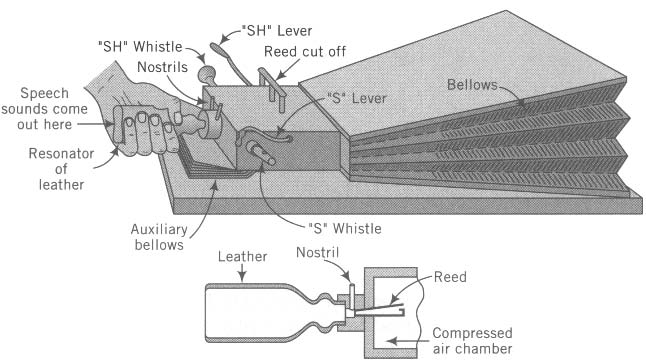
\includegraphics{vonKepelenSystem.jpg}
    \caption{Máquina de von Kempelen-Wheatstone}
    \label{fig:vonKempelenSystem}
\end{figure}

\begin{figure}[b]
    \centering
    \vspace{-13pt}
    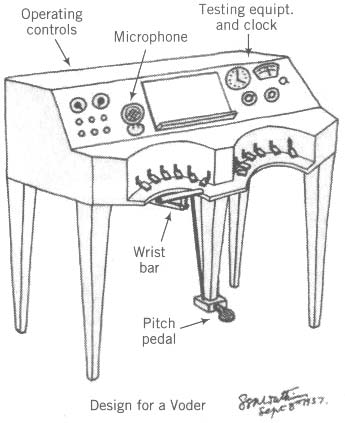
\includegraphics{dudley1939.jpg}
    \caption{Voder apresentador em 1939}
    \label{fig:dudley1939}
    % \vspace{-pt}
\end{figure}

\subsection{1939 - Homer Dudley e o Voder}
Anos mais tarde um pesquisador da \textit{Bell Telephone Laboratory}, Homer Dudley, buscou continuar a análise de von Kempelen em seus trabalhos \cite{doi:10.1121/1.1906583} \cite{goldSpeech} agora com os aparatos eletrônicos disponíveis. Em 1939 ele chamou a atenção do mundo ao apresentar na Grande Feira Mundial de 1939 de São Francisco e Nova Iorque o dispositivo chamado de \emph{Voder} (\textit{\textbf{Vo}ice-operated \textbf{De}monstrato\textbf{r}}). Esse dispositivo que pode ser visto na figura \ref{fig:dudley1939} produzia sons a partir dos movimentos do usuário sobre as pedaleiras, manivelas e ajustes que filtravam uma fonte de ruído, apresentando resultados como na síntese subtrativa. O \textit{Voder} não era capaz de produzir sons sem um habilidoso operador dada sua grande quantidade de parâmetros a serem controlados simultaneamente. Muitos dos operadores iniciados no treinamento não foram capazes de operar ou demoraram até um ano para conseguir manipular com destreza o aparelho. 

%QUESTION: Vale a pena introduzir o espectrograma do Voder aqui ou não? O espectrograma é uma ferramenta visual interessante para argumentar a performance dos diferentes tipos de modelo de síntese independente da sua tecnologia mas esse espectrograma fica isolado aqui até que seja apresentado outro para comparação. Talvez apresentar primeiro um histórico e tornar a visitar o espectrograma quando a comparação for ser feita?
%ANSWER: Vale sim! A introdução do espectrograma aqui ajuda a trabalhar a mesma ideia depois. Vale a pena explicar rapidamente a intuição do espectrograma mais pra frente no capítulo em uma outro seção

Comparando o espectrograma de um falante humano e de de um áudio gerado por um \textit{Voder} (Fig. \ref{fig:espectrograms}) percebemos que a síntese ainda não era capaz de capturar toda a riqueza do espectro humano especialmente nas harmônicas e frequências mais altas. O espectrograma é uma das ferramentas mais poderosas para observar o comportamento dos sintetizadores e comparar com a voz humana. Percebemos também que como o \textit{Voder} por ser operado por controles manuais apresentava fonemas naturalmente mais longos de modo que o operador fosse capaz de executá-los, outro fator para o forte sentimento sintético desse som.

\begin{figure}[t]
    \centering
    \begin{subfigure}[b]{\textwidth}
        \centering
        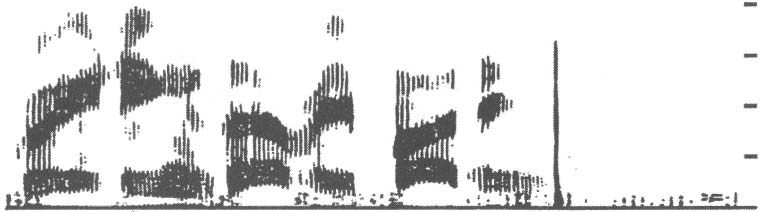
\includegraphics{g1.jpg}
        \caption{Humano}
    \end{subfigure}
    \begin{subfigure}[b]{\textwidth}
        \centering
        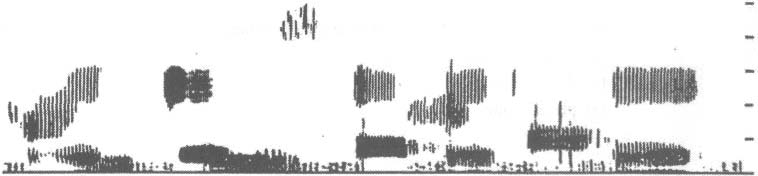
\includegraphics{g2.jpg}
        \caption{Voder}
    \end{subfigure}
    \caption{Espectrograma da frase ``greetings everybody"}
    \label{fig:espectrograms}
\end{figure}


%QUESTION: Vale a pena trabalhar que o sistema do Voder é baseado em sistemas de filtragem? O modelo foco do trabalho não lida com esse aspecto e ele não é exatamente relevante...
%ANSWER: Sim, vale a pena pois é fruto de conteúdo de pesquisa. Mesmo não agregando conteúdo direto ao trabalho agrega valor histórico

No início do século XX temos uma forte influência de Alan Turing para o interesse pela síntese de voz devido ao seu famoso Teste de Turing. A fala é um fator importante no teste de Turing completo onde haveria uma interação total entre a máquina e o usuário através de um robô. Nesse aspecto a fala deveria ser indistinguível de um falante humano para nos confundir perfeitamente. Turing apresentou sua tese em 1950 e alguns anos depois já existiam alguns projetos para síntese existentes. A ideia geral de diversos projetos pode ser observada na figura \ref{fig:voderIdea} (inclusive do próprio \textit{Voder} de Dudley) onde uma fonte de ruído é filtrada e ressoada de acordo com o interesse do usuário em produzir diferentes fonemas.

\begin{figure}
    \centering
    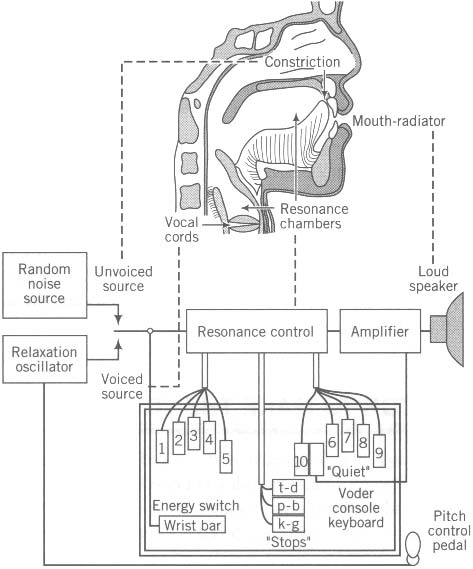
\includegraphics{voderIdea.jpg}
    \caption{Esquema de Filtragem de um \textit{Voder}}
    \label{fig:voderIdea}
\end{figure}


Em 1961 ainda na \textit{Bell Labs Technology} a pesquisa na síntese de fala iniciada por Dudley continuava e John Larry Kelly Jr. juntamente com Louis Gerstman usaram um IBM 704 para síntese. Um episódio popularmente conhecido foi a síntese de "Daisy Bell" gravada por eles ter sido ouvida por Arthur C. Clarke que visitava um colega. Arthur ficou tão impressionado com a tecnologia de fala que acabou tornando-se parte de sua obra \emph{2001: Uma Odisseia no Espaço} através do robô HAL 9000 \footnote{\url{https://www.youtube.com/watch?v=iwVu2BWLZqA}}.

\subsection{1970 - Gunnar Fant e a Síntese Articulatória}
Em 1970, Gunnar Fant publicou seu livro \textit{Teoria Acústica da Produção da Fala} \cite{fant1960acoustic} e nele defendeu um modelo de tubos para modelar a voz humana. Tomando como base o trato vocal como um todo é possível imaginar que seja um tubo aberto ou fechado na ponta dependendo de qual fonema esteja sendo produzido. Sua pesquisa baseou-se fortemente na observação de imagens de raio-x de pessoas falando os mais diversos fonemas.

Diversos cientistas além de Fant buscaram modelar matematicamente a voz ou o aparelho vocal como um todo mas dada a complexidade do sistema os resultados nunca não foram totalmente satisfatórios. A modelagem física sofreu diversas especulações até o aparecimento de tecnologias como o raio-x ou a a endoscopia que permitissem observar as cavidades internas em movimento. Outra forte crítica à modelagem física é que muitos deles focam apenas no trato vocal mas abstraem a importância de outras partes do corpo como a ressonância sofrida pela fala no crânio ou a amplitude da abertura do maxilar para produção da mesma.

\subsection{Síntese Concatenativa}
%QUESTION: Preciso introduzir esses três parágrafos trabalhando a questão da gravação? Da metodologia? Da faixa de compreensão da voz humana?
%ANSWER: É interessante apenas para pontuação referencial. Caso haja algum comentário negativo por parte da banca basta remover.

Em certo momento houve um interesse em gravar de alguma maneira instruções que pudesse ser replicada posteriormente para reprodução de um mesmo som. Tomando a mesma ideia dos cartões perfurados usados nos primeiros computadores criou-se uma pianola, que é um piano que lê um rolo responsável por apontar qual nota deve ser tocada e suas respectivas durações. 

Os primeiros fonógrafos e gramofones datam do final do século XIX com um mecanismo de cone para coletar as vibrações sonoras registradas através de uma membrana e com uma sensível agulha registrar essas vibrações de modo que pudessem ser replicadas e gerar o som novamente. Por diversos fatores os primeiros aparelhos eram bastante limitados e não eram capazes de capturar nem todo o conteúdo da nossa fala nem toda a faixa de frequência que somos capazes de ouvir. Nossa faixa de frequência audível está entre 20 e 20kHz, aproximadamente enquanto a voz flutua entre 50 e 3400Hz em geral. Os primeiros gravadores, no entanto, capturavam apenas a faixa entre 250 e 2500Hz aproximadamente o que compreende a quase 70\% da faixa representativa da voz.

A partir da evolução da gravação do som foi possível desenvolver a síntese concatenativa que, por ser originada completamente de um processo natural produzia resultados mais agradáveis ao ouvido do que os modelos matemáticos até então introduzidos.

\subsubsection{Unidades Mínimas}
\label{subsection:unidades_minimas}
%QUESTION:  Faz sentido já estabelecer um link aqui com os modelos sequenciais? Tratar as unidades mínimas como grams?
%ANSWER: Faz sim. Podemos citar e colocar a referência para a seção respectiva de modo a tentar o leitor numa leitura não linear

Na síntese concatenativa gravam-se diversas \emph{unidade mínimas} de um falante e as concatenamos para síntese posterior. Essas unidades mínimas variam de acordo com o sistema utilizado. Analisaremos primeiramente o padrão ocidental que nos é mais comum e então faremos alguns comentários sobre o padrão oriental com foco no japonês por ser uma língua com grande interesse na síntese de voz.

Usar cada letra como unidade mínima é trabalhoso e gera resultados imprecisos pois as letras apresentam diferentes comportamentos pareadas com umas e outras. O sistema de letra para fonema é frequentemente utilizado como suporte ao sistema de dicionário, que é o mais famoso. No sistema de dicionário uma grande quantidade de palavras tem seu(s) equivalente(s) fonético(s) representado(s) para consulta. Em geral a construção de um dicionário é trabalhosa por ter que traduzir tantas palavras de um formato para outro. Podemos citar dentre os dicionários o CMU Dict, organizado pela Carnegie Mellon University \cite{cmudict} e o dicionário fonético brasileiro Fala Brasil \cite{falabrasil} criado pelo grupo da UFPA em 2008. Outra pesquisa importante focada na geração de um sistema de conversão grafema para fonema é o PETRUS \cite{petrus} mas esse sistema é baseado em HMM treinado a partir do mesmo dicionário produzido pelo grupo do Fala Brasil \cite{hmm}.

Uma outra unidade mínima frequentemente citada na literatura é o fonema. O fonema é uma unidade mínima excelente pois existe uma quantidade finita e reduzida de fonemas mas muitos fonemas são influenciados pelos imediatamente anteriores ou posteriores de modo que a concatenação exclusivamente de fonemas acaba gerando aberrações e falhas prejudicando assim a síntese devido aos resultados artificiais. A síntese com unidades é de baixo custo computacional proporcional apenas ao esforço necessário apenas na junção das unidades. O custo computacional é contrastado porém com a grande massa de dados necessário para armazenar todas as unidades.

%QUESTION: Tratar de estratégias alternativas às unidades mínimas aqui? Introduzir outras técnicas de unidade mínima? Tratar da interpretabilidade delas já aqui? Introduzir as técnicas e comentar que a interpretabilidade será tratada posteriormente (com sua devida referência a uma seção posterior)?

Uma das propostas para reduzir o problema de aberrações nas junções de fonemas é a gravação de difonemas (tradução livre de \textit{diphone}) que são dois meio fonemas adjacentes. Pode ser entendido como a transição de fonemas e, desse modo, se torna um candidato que oferece estabilidade nas concatenações já que existe uma maior estabilidade na sustentação de um fonema do que na transição dos mesmos. A síntese a partir de difonemas ou apenas fonemas gera um banco de tamanho reduzido mas varia de tamanho de acordo com a linguagem apresentada (\textit{e.g.} a quantidade de fonemas de Coreano difere de Inglês). Além disso é possível aplicar técnicas de DSP (\textit{\textbf{D}igital \textbf{S}ignal} \textbf{P}rocessing) para adicionar prosódia, movimento e entonação reduzindo a monotonia da voz. Técnicas como PSOLA, por exemplo, alteram o timbre da fala e podem ser até usadas para manipular a voz em uma certa melodia, como é utilizada em diversas montagens com políticos cantando músicas populares \footnote{\href{https://www.youtube.com/user/baracksdubs}{https://www.youtube.com/user/baracksdubs}}.

Nos idiomas orientais a própria formação da língua auxilia a construção de sintetizadores com unidades mínimas de cada linguagem. O japonês, por exemplo, é composto de diversas unidades mínimas com sons bem determinados em seus alfabetos fonéticos (Hiragana (Fig. \ref{fig:hiragana}) e Katakana). O alfabeto de Kanjis expressa uma ideia ou palavra e não auxilia em nosso estudo.

\begin{figure}[ht]
    \centering
    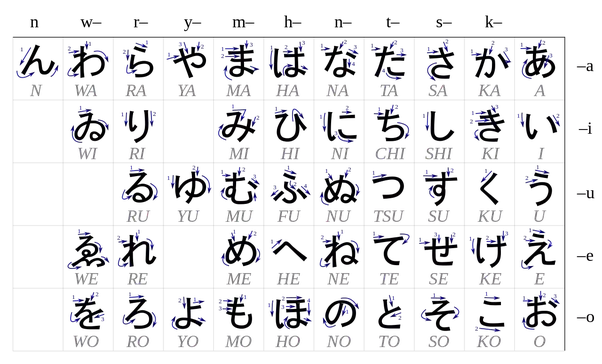
\includegraphics[width=0.9\textwidth]{main-qimg-1b1565ba8f6ec3e731ed623dba6e9d50.png}
    \caption{Alfabeto de Hiragana com Fonético Ocidental Respectivo}
    \label{fig:hiragana}
\end{figure}

Tendo em vista que as unidades são muito bem definidas é compreensível que o japonês tenha facilidade em adotar esse método de unidades naturalmente dada a estrutura natural da língua. Esse é um dos fatores mais importantes que devemos observar ao analisar o japonês como língua predominante nos idiomas de síntese com essa técnica.

A síntese com sentenças inteiras é a mais natural mas configura aplicações específicas demais para ser considerada como síntese e adota-se apenas o termo reprodução.

\subsection{Síntese de Formantes}
A síntese de formantes é interessante por não precisar de um falante para produzir amostras. Essa técnica se baseia em parâmetros que podem ser controlados como: frequência fundamental, níveis de voz e nasalamento do som no tempo. Através dessa parametrização esse sistema torna-se compacto e de baixo custo computacional mas traz com isso uma voz de sonoridade artificial. Mas ao mesmo tempo essa voz é mais facilmente inteligível em altas velocidades tornado-se uma vantagem para leitores de texto. Essa técnica é útil para sistemas com restrições de memória ou processamento. O controle total de todos os aspectos da síntese de formantes permite uma miríade de prosódias e entonações variando a expressão de sentimentos da voz sintetizada mas para isso requerem uma manutenção complexa de seus parâmetros no tempo.

\subsection{Aplicações e Interesse Comercial}
Atualmente diversos serviços cotidianos usam a síntese de fala com diferentes tipos de técnicas e unidades mínimas. Serviços de navegação muitas vezes misturam unidades mínimas de frases inteiras com instruções mais comuns e efetuam uma síntese concatenativa para leitura do nome de ruas. 

A Yamaha atualmente vende o sistema de Vocaloids que é extremamente popular no japão. Sua voz mais popular é a da Vocaloid Hatsune Miku cuja popularidade extendeu-se de tal maneira que a voz ganhou um rosto, um modelo tridimensional e teve até apresentações em estádios em união ao artifício da projeção holográfica.

A síntese também é vendida como um serviço de terceiros, onde o interesse não é o modelo ou a técnica utilizada e sim métricas de negócio como volume de requisições, tempo de síntese, aplicabilidade no negócio, entre outros. Dos modelos comerciais que gabam dessas características e efetivamente afirmam utilizar modelos de rede neural (por mais que não explicitem os modelos) são o Amazon Polly \cite{polly} e o Google Cloud Text-to-Speech \cite{cloud_tts}. O Google utiliza efetivamente o serviço de síntese em outros de seus serviços como o Google Tradutor, Assistente e mais recentemente demonstrou o projeto Duplex que é capaz de interagir em todo o processo de compreensão, síntese e interação para uma dada atividade. 

Avançando ao ferramental comercial interessado na síntese genérica de qualquer falante tivemos em 2016 a Adobe que exibiu na sua própria conferência um protótipo de aplicação chamada Adobe VoCo\footnote{\url{https://theblog.adobe.com/lets-get-experimental-behind-the-adobe-max-sneaks/}} com propriedades de edição similar a outros editores de áudio mas com a capacidade de sintetizar perfeitamente sentenças não faladas por um dado falante com uma quantidade mínima de áudio para treino e logo em seguida a fundação da startup canadense lyrebird\footnote{\url{https://lyrebird.ai/}} fundada por estudantes da MILA (University of Montreal - Montreal Institute for Learning Algorithms) pupilos do Yoshua Bengio, um dos patronos de vários artigos importantes na área de redes neurais. A simples sugestão de tais aplicações gerou uma grande preocupação quanto à possíveis má utilizações e a falta de assinaturas ou métodos que permitissem a verificação de tais sínteses. Enquanto não desenvolveu-se uma solução para esse problema houve continuidade de pesquisa apenas no meio acadêmico. 

Cronologicamente temos a constante participação de grandes empresas na continuidade da pesquisa pela síntese de fala genérica como podemos ver na organização de trabalhos abaixo:


\begin{itemize}
    \item Em Setembro de 2016 o \textbf{Google} publicou o primeiro resultado do WaveNet \cite{wavenet} que seria o primeiro modelo neural responsável pela síntese de áudio;
    \item Em fevereiro de 2017 o \textbf{Baidu} publicou resultados do Deep Voice \cite{deepVoice} que seria o primeiro modelo completamente composto por redes neurais a atingir a síntese de fala;
    \item Em março de 2017 o \textbf{Google} publicou a primeira versão de seu modelo de síntese de fala ponta a ponta, o Tacotron \cite{tacotron}
    \item Em maio de 2017 \textbf{Baidu} novamente publicou resultados do seu modelo Deep Voice melhorado nomeando-o Deep Voice 2 \cite{deepVoice2}. Houve melhorias de performance no treinamento devido a um kernel implementado diretamente nas GPU contornando assim os gargalos presentes nas trocas de informação com os frameworks anteriormente utilizados;
    \item Em julho de 2017 o \textbf{Facebook} publicou o VoiceLoop \cite{facebook:DBLP:journals/corr/TaigmanWPN17}\footnote{\url{https://research.fb.com/publications/voiceloop-voice-fitting-and-synthesis-via-a-phonolgoical-loop/}}, o foco desse trabalho foi a síntese a partir de exemplos naturais, ou seja, sem se preocupar com a correlação de sinal-ruído;
    \item Em outubro de 2017 \textbf{Baidu} publicou a versão final de seu modelo Deep Voice, o Deep Voice 3. Esse modelo usou um sistema mais simples que os anteriores o que fez com que seu treino e inferência fossem mais rápidos e a convergência do modelo pudesse ser obtida mais rapidamente já que haviam menos parâmetros a otimizar. Esse modelo também se utilizou largamente de convoluções permitindo uma alta paralelização;
    \item Em dezembro de 2017 o \textbf{Google} publicou o Tacotron 2\cite{tacotron2:DBLP:journals/corr/abs-1712-05884}, uma versão incrementada do modelo apresentado no início do mesmo ano.
    \item Em Fevereiro de 2018 o \textbf{Baidu} \cite{baidu_voice_clonning:DBLP:journals/corr/abs-1802-06006} reavaliou seus modelos anteriormente publicados para confrontar o modelo do Facebook nesse trabalho focou em desenvolver uma solução de readaptação dos modelos anteriores
\end{itemize}

Todos esses modelos compartilham das mesmas ideias construídas e dissecadas nos modelos de síntese estudados anteriormente. Gostaria de usar nesse trabalho uma implementação do modelo do Deep Voice cujo modelo básico pode ser visto na Fig. \ref{fig:deep_voice_blocks}. O intuito desse trabalho é observar especificamente a alteração do idioma de entrada que confere um impacto maior na rede de entrada, no caso, o modelo grafema para fonema que tem suas entradas alinhadas ao modelo de segmentação. Esse modelo tem como responsabilidade fazer a conversão de todo texto de entrada para algum modelo fonético (como o IPA ou o SAMPA) assim como alinhar esses símbolos escolhidos para alguma sequência de áudio de entrada. O modelo treinado nesses casos é um modelo de atenção que será detalhado na seção \ref{sec:redes}. O modelo responsável pela síntese é o WaveNet. O modelo de extração de F0 da voz é treinado com uma outro algoritmo de extração de frequência fundamental para cada segmento determinado.


\begin{figure}
    \centering
    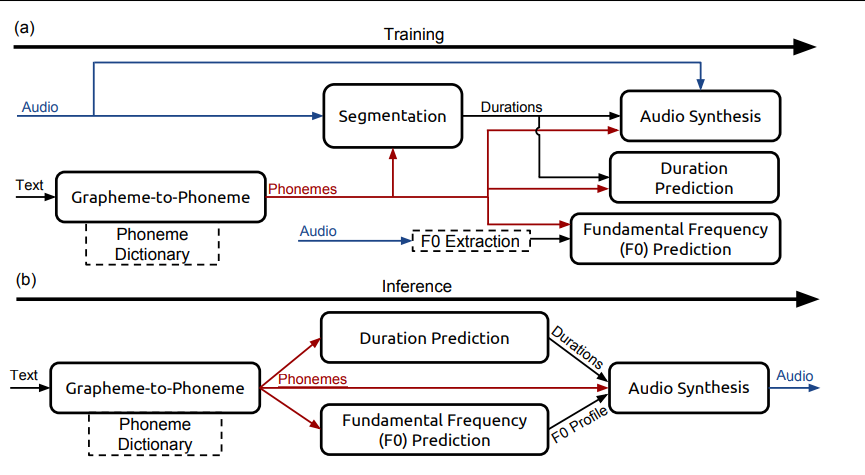
\includegraphics[width=\textwidth]{figuras/blocos.png}
    \caption{Blocos de Síntese do Deep Voice}
    \label{fig:deep_voice_blocks}
\end{figure}


\section{Alfabetos Fonéticos}
A quantidade de fonemas possíveis de serem expressados pelo trato vocal humano é finito. Não é comum uma linguagem se utilizar de todos os fonemas possíveis na fala humana e a presença de uma quantidade maior ou menor de fonemas também acaba determinando a facilidade de se aprendê-la.

Para garantir uma internacionalização linguisitas criaram o IPA (\textit{International Phonetic Alphabet}) que pode ser consultado na tabela no Apêndice \ref{ape:ipa}. Esse alfabeto vem passando por constantes revisões desde sua criação inicial em 1886. Devido a presença de diversos símbolos fora do padrão latino houve a necessidade da criação de um outro alfabeto que servisse de conversão intermediária e pudesse ser facilmente lido por computadores (anterior à implementação do padrão UTF-8). Para a fácil interpretação dos computadores foi criado o alfabeto SAMPA que consiste na mesma ideia de representar a fonética humana com símbolos mas o foco agora foi a fácil implementação nos computadores.

Um dos maiores dicionários fonéticos em inglês, o CMU Dict\cite{cmudict}, se utiliza desse padrão SAMPA. Através da análise de um dicionário fonético temos como observar a frequência de fonemas relativos em uma linguagem e assim estabelecer uma comparação a outra linguagem. 

%inserir análise CMU Dict vs Dicionario PT https://github.com/falabrasil/phonetic-dicts

Uma comparação apenas por dicionário pode não ter impacto no balanço de fonemas utilizados efetivamente na fala, assim observamos a frequência relativa dos fonemas efetivamente utilizados na análise abaixo

% LJSpeech vs Vox vs Cellbit

\begin{figure}
    \centering
    \begin{subfigure}[c]{0.6\textwidth}
        \centering
        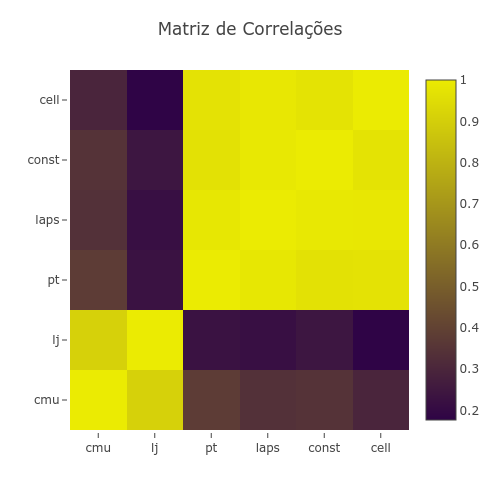
\includegraphics[width=\textwidth]{figuras/corr_phonemes.png}
        \caption{Mapa de Temperatura}
    \end{subfigure}
    ~
    \begin{subtable}{0.5\textwidth}
        \centering
        \begin{tabular}[c]{|r|cccccc|}
        \hline
        {} &        cmu &         lj &         pt &       laps &      const &       cell \\
        \hline
        cmu   &       1.00 &       0.91 &       0.38 &       0.34 &       0.35 &       0.29 \\
        lj    &       0.91 &       1.00 &       0.23 &       0.22 &       0.24 &       0.18 \\
        pt    &       0.38 &       0.23 &       1.00 &       0.98 &       0.96 &       0.97 \\
        laps  &       0.34 &       0.22 &       0.98 &       1.00 &       0.99 &       0.99 \\
        const &       0.35 &       0.24 &       0.96 &       0.99 &       1.00 &       0.97 \\
        cell  &       0.29 &       0.18 &       0.97 &       0.99 &       0.97 &       1.00 \\
        \hline
        \end{tabular}
        \caption{Matriz de Correlação}
    \end{subtable}
    \caption[Correlação entre Datasets]{Observando a matriz de correlação observamos alta correlação nos fonemas de uma mesma língua nos conjuntos de dados.}
    \label{fig:corr}
\end{figure}

\begin{figure}
    \centering
    \begin{subfigure}[c]{\textwidth}
        \centering
        \vspace{-40pt}
        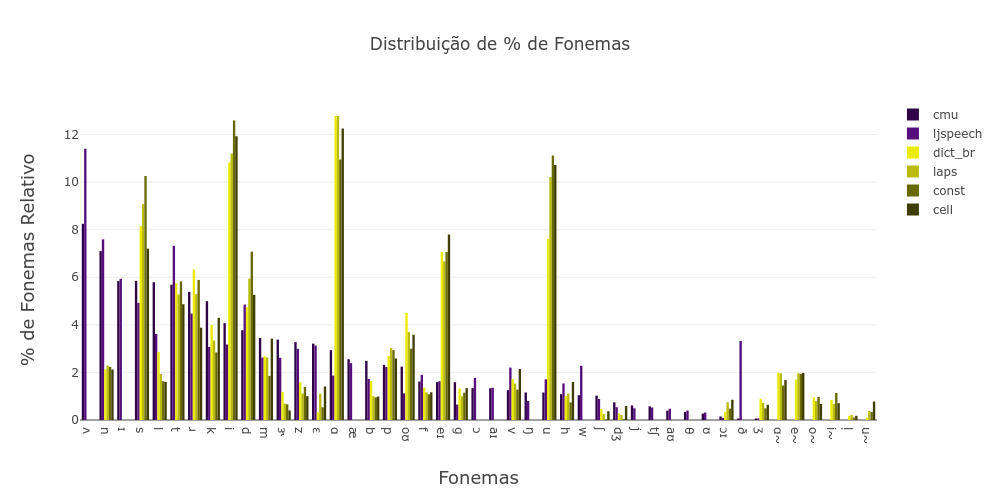
\includegraphics[width=\textwidth]{figuras/bar_all_phonemes.png}
        \caption{Participação Relativa em Todas as Línguas}
    \end{subfigure}
    \begin{subfigure}[c]{\textwidth}
        \centering
        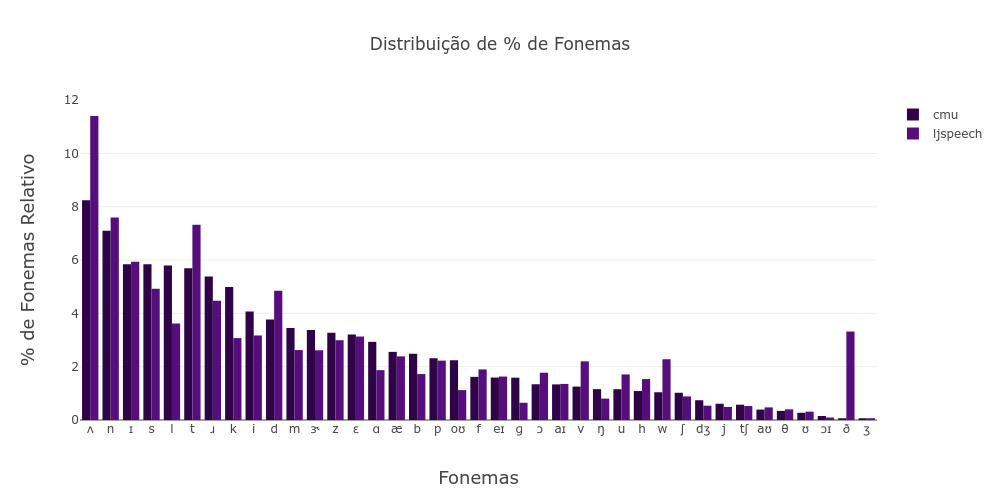
\includegraphics[width=\textwidth]{figuras/bar_en_phonemes.png}
        \caption{Participação Relativa no Inglês}
    \end{subfigure}
    \begin{subfigure}[c]{\textwidth}
        \centering
        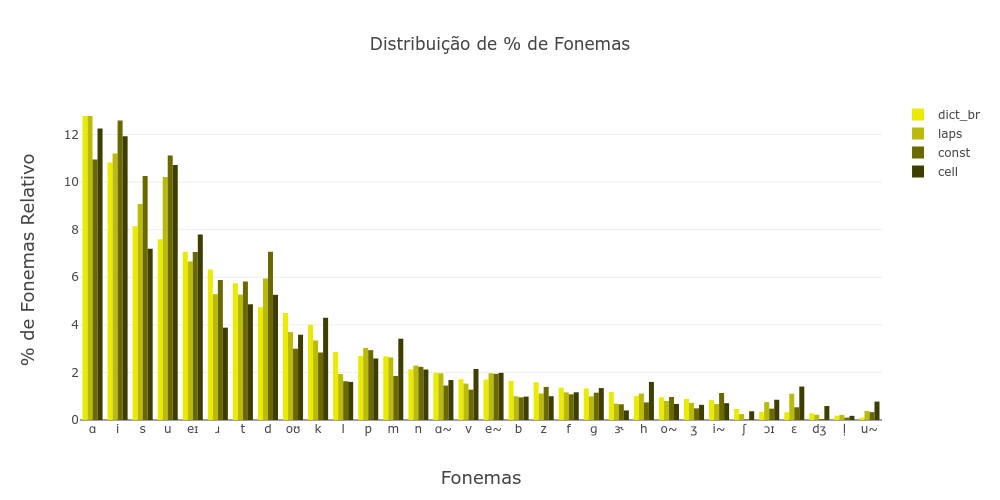
\includegraphics[width=\textwidth]{figuras/bar_pt_phonemes.png}
        \vspace{-20pt}
        \caption{Participação Relativa no Português}
    \end{subfigure}
    % \vspace{-20pt}
    \caption{Distribuição de Fonemas por conjunto de dados}
    \label{fig:fonemas_analysis}
\end{figure}
% https://pandas.pydata.org/pandas-docs/stable/reference/api/pandas.DataFrame.corr.html
LJSPeech
% https://keithito.com/LJ-Speech-Dataset/

Para a análise tomamos dois dicionários fonéticos, um em inglês e um em português, e alguns conjuntos de falas transcritas que utilizaremos no processo de treino. Usamos como base para o inglês o LJSpeech e para o português três conjuntos de fala: o LAPS, a Constituição, ambos fornecidos pelo projeto FalaBrasil, e o conjunto de fala extraído de vídeos do youtube, conforme detalhado na seção \ref{sec:youtube}.

Para montar a análise entre línguas utilizamos um método de conversão apontado pela tabela de fonemas internacional, disponível no Apêndice \ref{ape:ipa}. Dessa forma garantimos o alinhamentos dos fonemas corretos entre idiomas. Para a análise dos trechos falados fomos restritos ao alinhamentos das transcrições disponíveis com os respectivos dicionários de cada língua. Naturalmente esse foi um processo com perdas conforme apontado abaixo:
\begin{enumerate}
    \item LJSpeech - Perda de 01139 palavras, correspondente a 08.28\%
    \item LAPS - Perda de 00046 palavras, correspondente a 01.68\%
    \item Constituição - Perda de 00526 palavras, correspondente a 09.87\%
    \item YouTube - Perda de 03344 palavras, correspondente a 50.08\%
\end{enumerate}

Podemos perceber que muitos dos termos obtidos dos dados do youtube não foram alinhados com algum termo do dicionário. Isso tem raiz no grande uso de neologismos, aumentativos, diminutivos, estrangeirismos e outras formas de variação da linguagem formal.

\section{Redes Neurais e Aprendizado de Representações}
\label{sec:redes}
O tópico redes neurais gera grande confusão naqueles que são novos no campo por englobar muitas técnicas com diferentes finalidades. O intuito desse trabalho não é dissertar sobre todos os aspectos que compõem o campo de Aprendizado Profundo (\textit{Deep Learning}), Redes Neurais ou do conceito geral de Aprendizado de Representações. Apresentaremos nessa seção um breve resumo dos blocos importantes à compreensão deste trabalho pontuados por referências onde o leitor pode encontrar um detalhamento maior dos mesmos além de diversos outros tópicos relacionados nesse conjunto de técnicas.

Este trabalho pensa na sequência de letras, fonemas, palavras e sons como uma cadeia temporal sequencial de informações. A literatura de técnicas para cadeias temporais tem origem no interesse de se trabalhar com texto. Como o próprio trabalho se propõe a receber uma entrada de texto damos a intuição das técnicas também com texto.

\subsection{Representações Densas}
Um dos problemas básicos para tratar palavras em aprendizado de máquina é a dificuldade de se obter um padrão das mesmas como entrada para os algoritmos. Quando lidamos com texto usualmente não temos um tamanho de sequência bem definidas. No contexto de palavras temos palavras com diferentes tamanhos e no contexto de frases temos sentenças com diferentes comprimentos. 

Uma das primeiras técnicas usadas foi a construção de um vetor de contagem de palavras. Nessa técnica cada sentença é abstraída em um vetor esparso com comprimento do vocabulário do corpus. Essa técnica mitiga o problema de falta de padrão pois todas as palavras teriam alguma representação vetorial com uma mesma dimensão. O problema dessa técnica além da dificuldade de se lidar com vetores esparsos é a completa ortogonalidade entre todos os termos, isso é, assume-se que todas as palavras seriam completamente independente umas das outras. Essa premissa é claramente falsa quando pensamos na morfologia e sintaxe da nossa língua. Isso também acontece quando observamos os fonemas que são divididos em classes de acordo com o som que produzem e da maneira que são produzidos.

Palavras que compartilhem uma mesma característica morfológica ou que possuam proximidade semântica poderiam estar agrupadas em um mesmo grupo de contextualização. Baseado nessa ideia podemos pensar que em um corpus grande suficiente teríamos uma quantidade razoável de relações semânticas para ser aprendidas. Essa é a intuição do word2vec \cite{word2vec:DBLP:journals/corr/MikolovSCCD13} onde temos duas técnicas de aprendizado: a CBOW (Cumulative Bag of Words) e a SkipGram. Na CBOW várias palavras são alimentadas e buscamos prever uma única palavra de contexto enquanto na SkipGram a palavra de contexto é alimentada e buscamos prever as palavras dentro daquela janela. O intuito dessa técnica é exatamente tentar capturar a semântica das palavras baseado nas palavras que aparecem próximas a ela. Esse tipo de semântica só pode ser bem generalizado em corpus grandes tendo em vista as mais diversas situações que uma mesma palavra poderia se relacionar com outras. A utilização de corpus pequenos tende a gerar modelos pouco genéricos que acabam englobando apenas um pequeno domínio. 
% No word2vec a função objetivo que desejamos minimizar é a perplexidade descrita na equação \ref{eq:preplexity}.

Outras técnicas incrementaram pontos fracos do word2vec como a Glove \cite{glove:pennington2014glove} ou fastext \cite{fasttext:joulin2016fasttextzip}. Essas técnicas são comumente usadas para capturar relações entre palavras mas podem ser usadas em outros níveis também, com a nível de caracter, sentença, parágrafo, entre outros. No caso do nosso problema esse módulo é responsável por capturar uma representação própria para a palavra visando sua representação fonética. Para agregar essa informação precisamos de outra célula, a célula recorrente.

\subsection{RNN - Redes Neurais Recorrentes}
As células recorrentes foram pensadas para capturar informações em uma dada cadeia de dados. Elas funcionam como os neurônios simples clássicos mas uma das entradas que recebem é também a saída da iteração do passo anterior (Fig. \ref{fig:rnn}).

\begin{figure}[h]
    \centering
    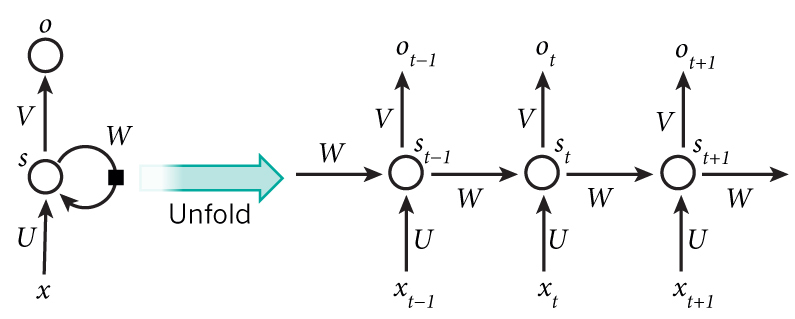
\includegraphics[width=0.9\textwidth]{figuras/rnn.jpg}
    \caption{Célula Recorrente}
    \label{fig:rnn}
\end{figure}

No entanto essas células inserem um desafio computacional quanto à complexidade de sua propagação de erros. Comumente nos neurônios simples existe uma função bem definida cujo comportamento pode ser ajustado através do algoritmo de propagação retroativa de erros (\textit{backpropagation}) mas ao adicionarmos uma dimensão extra (tendo em vista que é uma sequência) a propagação sofre um problema. O primeiro problema fácil de perceber é que a medida que as sequências ficam mais longas a propagação demora cada vez mais para atingir o início da sequência dada a necessidade de se recalcular os gradientes com os erros para cada passo anterior do tempo na sequência. O segundo problema provém do mesmo problema onde caso a o módulo da matriz de pesos seja maior que 1 o gradiente explode à medida que é propagado e não somos capazes de aprender nada (\textit{exploding gradient}) caso o módulo seja menor que 1 o problema oposto ocorre onde o erro propagado rapidamente tende a 0 e ficamos incapazes de propagar erros mais que alguns passos no passado (\textit{vanishing gradient}). O comportamento do gradiente pode ser controlado a partir da matriz de inicialização dos pesos no passo inicial. Desde que a inicialização seja bem calculada com valores que evitem a explosão e a inércia dos valores. \cite{exploding_gradient}

Numa célula RNN tradicional toda informação é passada para a célula seguinte. Isso torna sequências muito longas ou cujas informações relevantes sejam necessárias vários passos depois muito difíceis de codificar. Uma tentativa de se controlar a quantidade de informação passada em cada passo foram as unidades GRU (\textit{Gated Recurrent Unit}) e LSTM (Long Short Term Memory). Essas duas unidades (Fig \ref{fig:gated_units}) possuem sistemas de passagem parcial de informações, seus portões, cujos parâmetros também são aprendidos durante o treino. A medida que acrescentamos parâmetros numa célula geramos uma crescente sobrecarga de informações a serem computadas em cada passo de modo que essa técnica possui um custo computacional no treinamento do modelo. 

\begin{figure}[h]
    \centering
    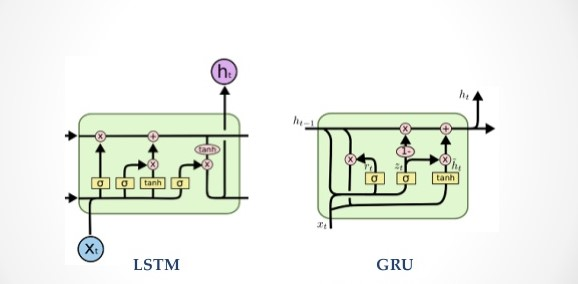
\includegraphics[width=0.9\textwidth]{figuras/recurrent_cell.jpg}
    \caption{Células Recorrentes}
    \label{fig:gated_units}
\end{figure}


\subsection{Conectist Temporal Classification (CTC) e Beam Search}
Em um modelo encoder-decoder o decoder pode ter algumas estratégias para executar o processo de decodificação. A mais simples é predizer apenas um valor (seja ele uma classe ou um valor regredido). Essa abordagem é bastante agressiva pois qualquer classificação errônea seria propagada pelo modelo de decodificação. Uma estratégia pensada para contornar esse problema é a predição das melhores classes que se adéquem a algum limiar. Desse modo cada passo pode predizer várias classes e a saída fica sendo a sequência de probabilidades das classes a serem preditas. Ao final da predição da cadeia analisa-se essa sequência e montamos a saída através de uma programação dinâmica onde busca-se maximizar as probabilidades entre as unidades. 

Tomando um exemplo de tradução por exemplo podemos ter o seguinte exemplo: o encoder codifica a palavra em português "gato" para um vetor intermediário denso; o decoder com CTC pode decodificar esse vetor de várias maneiras como podemos ver abaixo, onde o espaço de quebra de letra é o $<b>$:
\begin{itemize}
    \item $ccc<b>a<b>ttttt<b>$
    \item $c<b>aaa<b>tt<b>$
    \item $ccc<b>aaoaa<b>t<b>$
\end{itemize}
Através do algoritmo de programação dinâmica Beam Search buscamos maximizar a probabilidade da predição da cadeia. O algoritmo busca maximizar a probabilidade dentre as unidades previstas de se alinharem entre um mesmo bloco e entre blocos. Cada bloco é o conjunto de predições que não foram quebradas por um caracter de quebra ($<b>$). Assim também conseguimos propagar os gradientes na rede e somos capazes de mapear todas as sequências para a palavra "cat". Mesmo classificações incorretas em algum tempo podem ser corrigidas pela maximização de probabilidade de cada letra, no caso.

As unidades mínimas típicas de texto são letras e palavras. O alinhamento do encoder-decoder num sistema de tradução neural é então de letra para letra ou de palavra para palavra. No nosso modelo grafema-fonema a entrada do modelo é texto e a saída é fonema. O alinhamento ocorre com os trechos de palavra conhecidos com algum fonema previsto na saída. O mesmo princípio explicado acima com letras se verifica e os fonemas são alinhados a uma saída seccionando a entrada paralela a um trecho respectivo de texto e som.


\subsection{Convoluções Autoregressivas Dilatadas}
O modelo de síntese mais popular atualmente é o WaveNet \cite{wavenet}. O intuito desse módulo é oferecer uma alternativa à concatenação de unidades de síntese mínimas utilizadas. Na concatenação tradicional ocorrem aberrações fruto da natureza seccionada das unidades mínimas.

No modelo do WaveNet a geração de amostras de áudio é probabilística e atrelada as amostras anteriores. Comparativamente pode-se pensar que esse modelo utiliza uma unidade mínima como a unidade do áudio amostrado sem tratamento. Podemos perceber que isso trás um problema similar ao do gradiente nos modelos recorrentes pois as sequências de áudio com alta taxa de amostragem acabam sendo muito longas mesmo para poucos segundos de áudio. Para contornar esse problema o trabalho propôs duas técnicas combinadas: a utilização de uma janela onde apenas alguns passos anteriores seriam considerados na síntese de uma nova amostra; e a utilização das próprias saídas nas entradas de modo a eliminar as possíveis anormalidades presentes na transição de unidades.


\begin{figure}[h]
    \centering
    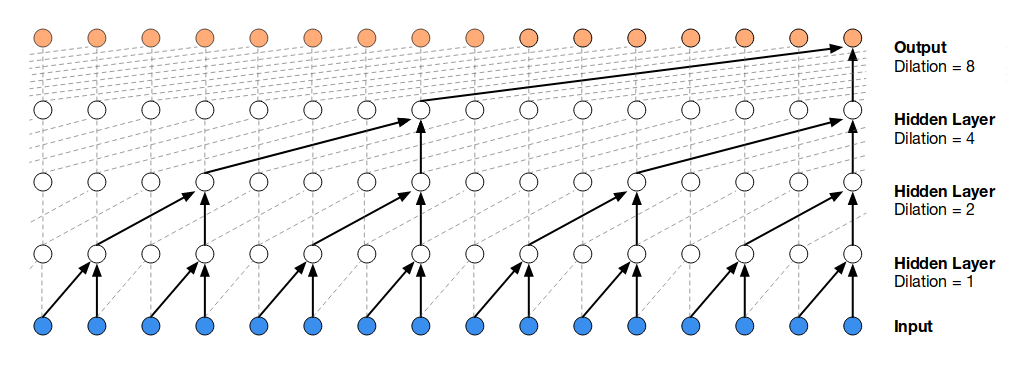
\includegraphics[width=0.9\textwidth]{figuras/dilataded_conv.png}
    \caption{Convolução Dilatada}
    \label{fig:dilatated}
\end{figure}

A primeira técnica efetua convoluções dilatadas (Fig \ref{fig:dilatated}) onde a convolução é aplicada  com espaçamentos de acordo com o valor alocado. O caso especial onde a dilatação é 1 configura a convolução tradicional.

A segunda técnica consiste numa estratégia que remete aos modelos de recorrência pois utiliza cada saída como entrada para as convoluções futuras. Essa estratégia pode ser executada rapidamente no treino do modelo pois as entradas são facilmente paralelizáveis e o modelo pode efetuar diversas operações de convolução simultaneamente. Entretanto quando essa estratégia é utilizada para predição é necessário esperar a geração de cada amostra para computar as amostras posteriores removendo o fator paralelizável e tornando-se um gargalo para a síntese em tempo real. Propostas posteriores \cite{deepVoice, wavenet_parallel:DBLP:journals/corr/abs-1711-10433} buscaram outras estratégias para alcançar performances melhores de tempo de execução do modelo



% \section{TTS como Produto}
% * Vocaloid (Hatsune Mike)
% * Amazon Polly https://aws.amazon.com/polly/?sc_icampaign=Adoption_Campaign_pac_paas_q3-07-2018_polly_sign_in&sc_ichannel=ha&sc_icontent=awssm-1046&sc_ioutcome=Product_Adoption_Campaigns&sc_iplace=signin&trk=ha_awssm-1046-ha_a131L000005jqNlQAI&trkCampaign=pac_polly_product_page
% * Google Translator


% \begin{wrapfigure}{r}{0.5\textwidth}
%     \centering
%     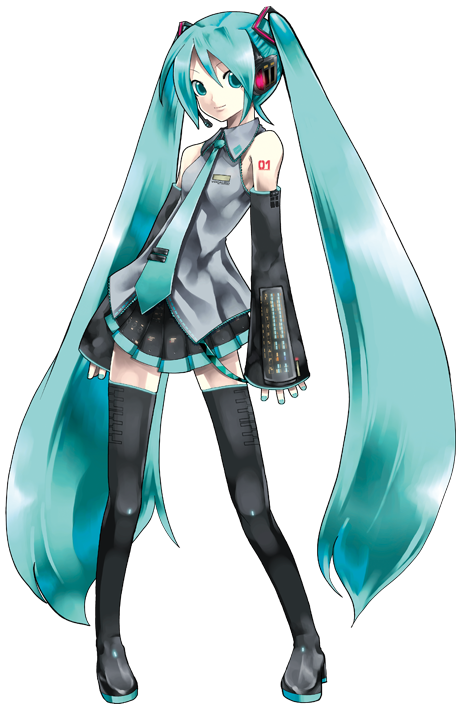
\includegraphics[width=0.5\textwidth]{Hatsune2.png}
%     \centering
%     \caption{Hatsune Miku, a famosa cantora virtual da série VOCALOID}
%     \label{fig:miku}
%     \vspace{-30pt}
% \end{wrapfigure}
% \section{Prosódia, Naturalidade, Entonação e }
% Os sistemas até esse ponto não eram capazes de funcionar automaticamente. O folde de von Kempelen produzia poucos fonemas e existia uma dificuldade muito grande em manipular o fole e alterar os ajustes para produção dos sons; O \textit{Voder}, por sua vez, precisava de um especializado operador para síntese; A modelagem de tubos de Fant, assim como von Kempelen, sofreram com a baixa quantidade de fonemas representados facilmente por seus sistemas. 

% Apenas com as sínteses concatenativas e de formantes foi possível sintetizar pela primeira vez todo conjunto de unidades para apresentar sistemas completos. Na síntese concatenativa o processo pôde ser então automatizado mais facilmente já que consistia apenas em utilizar as unidades previamente adquiridas e na síntese de formantes o desafio era manipular corretamente os poucos parâmetros de modo a estimular corretamente a síntese.

% Atingido aqui um primeiro momento da síntese de fala onde finalmente aprensentaram-se sistemas capazes de solucionar o problema aparecem outros tantos desafios para os sistemas de TTS como a entonação (como prosódia ou sotaques), a tradução do texto em fonemas (para utilização em sistemas concatenativos) e a criação de modelos que variassem no tempo conforme um falante específico (para determinar as entradas da síntese de formantes).

% A tradução do texto em fonemas é um desafio dadas diversas formas de se falar uma mesma palavra seja por regionalismos (extra com e aberto, como em Édipo, ou com e fechado, como em Êxito), seja por homografia (colher pode ter tônica no 'o' e ser respectivo ao verbo colher como em "vou colher batatas" ou pode ter tônica no 'e' e ser respectivo ao utensílio usado para comer). A esse novo desafio que aparece à síntese de voz de tratar também o texto chamamos \textit{normalização do texto} ou \textit{tokenização}. A especificação gerada por essa camada contem muitas camadas de informação como o texto original, o padrão de prosódia entre vários outros. A parte responsável por manipular os segmentos de voz para a partir dessas informações para geração da sonde de som ainda recebe o nome de síntese.



% Existe um grande desejo na comparação de diferentes técnicas. Usualmente analiza-se similaridade com a voz humana e a capacidade de ser compreendido sem dificuldade. Mas muito do fim influencia na melhor técnica a ser usada. Diversas técnicas de formantes soam extremamente artificiais mas são facilmente inteligíveis em alta velocidade em contraste com outras tecnologias. O tamanho do banco de dados também influencia a qualidade da voz assim como restringe o sistema. Temos em sistemas com muitas unidades uma excelente qualidade mas um grande tamanho de banco ou temos poucos fonemas gravados e a necessidade de manipulação de sinais para concatenar os poucos sinais e manipular a prosódia.


% \section{Síntese no Futuro}
% Com a apresentação em 2016 da Adobe de seu produto Adobe Voco, o software de edição e geração de áudio, chamado carinhosamente de Photoshop do áudio refletindo o sucesso desse outro produto da empresa. O assombro na apresentação do produto foi a pequena quantidade de amostra de áudio necessária (apenas 20 minutos na apresentação) para simular a prosódia e frequência fundamental \cite{voco2017}. Resultados similares foram obtidos com os trabalhos da Google com a WaveNet \cite{wavenet} e o Tacotron \cite{tacotron}, da Baidu com o Deep Voice \cite{deepVoice} e Deep Voice 2\cite{deepVoice2} com a utilização de redes neurais para a parametrização de diversos aspectos do processo de síntese em subsistemas. O problema de conversão de grafema para fonema é resolvido com uma maneira similar ao HMM comentado anteriormente, ou seja, através de um treinamento a partir de um dicionário da linguagem e então a utilização do modelo para separação dos fonemas. A síntese dos últimos 3 artigos se dá com a WaveNet que é uma rede que gera uma amostra de áudio por vez, dessa forma a descrição do artigo original precisa gerar muitas amostras para sintetizar alguns segundos de áudio (tendo em vista as taxas de amostragem mais baixas serem em torno de 8000 amostras por segundo teremos que sintetizar 8000 amostras com a rede para obter um segundo de áudio).

% O grupo de pesquisa do Baidu orientado por Andrew Ng desenvolveu algumas melhorias na síntese proposta pela WaveNet para otimizar a síntese e acelerar a mesma. A síntese proposta por Ng et al. não tomava uma quantidade tão grande de amostras anteriores para sintetizar cada nova amostra e isso acelera o processamento da rede sem afetar gravemente o resultado final, possibilitando (com outras tantas melhorias) a síntese em tempo real na Deep Voice 2. Ng et al. criticou o aprendizado de apenas parâmetros particulares de cada falante uma vez que a voz humana compartilha muitas características entre os falantes de todo mundo e por isso nas publicações mais recentes usou como massa de dados amostras de falantes anotadas de diversas nacionalidades, gêneros e idades permitindo à rede generalizar uma voz a ser sintetizada a partir de todas as outras e, quando fosse de interesse gerar uma voz específica, aplicar um ajuste fino dos parâmetros nesse modelo de maneira muito mais rápida.

% O foco central dessas pesquisas é apenas na síntese falada mais natural possível com algoritmos que apresentaram excelentes resultados em outras áreas. A adição de uma camada intermediária como a presente em pesquisas de transferência de estilo \cite{style} pode ser vital para a metamorfose completa de um áudio sintetizado para uma música com outro cantor ou com outra emoção. Tendo em vista a variedade de algoritmos e sistemas para síntese, a facilidade com que podemos editar, gravar e usar áudios para dar origens a novos sons estamos mais perto do que nunca de um controle completo sobre a síntese de uma voz humana indistinguível para os mais diversos fins.
% \begin{figure}[ht]
%     \centering
%     \begin{subfigure}[b]{\textwidth}
%         \centering
%         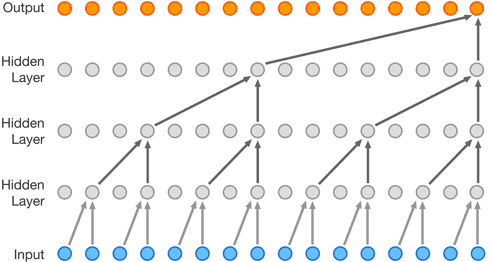
\includegraphics[width=0.6\textwidth]{wavenet.jpg}
%     \end{subfigure}
%     \begin{subfigure}[b]{\textwidth}
%         \centering
%         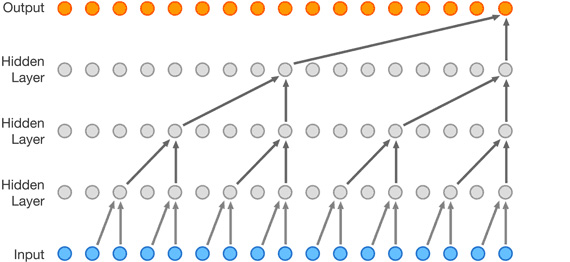
\includegraphics[width=0.7\textwidth]{wavenet2.jpg}
%     \end{subfigure}
%     \caption[Esquema de Síntese da WaveNet]{Esquema de Síntese da WaveNet utilizando amostras geradas sucessivamente para produçao das amostras futuras}
%     \label{fig:wavenet}
% \end{figure}